\documentclass[../tesis_main.tex]{subfiles}


\chapter{Resultados y conclusiones}

La descripción de las pruebas y la discusión de resultados se abordará con la siguiente estructura. Se describirán pruebas que permitieron realizar una evaluación del desepeño de los algoritmos con respecto a los que actualmente están operando en el robot de servicio Justina.\\

Se describirá conforme al desarrollo de este estrabajo. 

\begin{enumerate}
	\item{Extracción de planos.}
	\begin{itemize}
		\item{Exactitud, rapidez.}
	\end{itemize}

	\item{Extracción de objetos y sus características.}
	\begin{itemize}
		\item{Exactitud en la estimación de la posición.}
		\item{Comparación en caracteristica de altura.}
		\item{Estimación de la orientación de objetos.}
		\item{Exactitud en el cálculo de la orientación. Comparación orientación estimada y real.}
	\end{itemize}


	\item{Espacio de trabajo del algoritmo númerico.}
	\item{Prueba de tarea de manipulación con adición de la información de dimensiones.}
	\item{Comparación tarea de manipulación utilizando información de orientación de los objetos.}
\end{enumerate}





%%%%%%%%%%%%%%%%%%%%%%%%%%%%%%%%%%%%%%%%%%%%%%%%%%%%%%%%%%%%%%%%%%%%
%%%%%%%%%		EXTRACCIÓN DE PLANOS           %%%%%%%%%%%%%%%%%%%%%

	\section{Extracción de planos.}

	En esta sección analizaremos los resultados obtenidos al probar el algoritmo RANSAC para encontrar planos modificando el numero de iteraciones. Observaremos el comportamiento del error y el tiempo de ejecución a fin de encontrar el número óptimo de iteraciones para este algoritmo.\\

	El proceso para el análisis de datos fue el siguiente: se propuso un modelo de plano conocido por el usuario. Dicho modelo se obtuvo a partir del conocimiento de la altura del plano en este caso una mesa. Posteriormente se cuantificó la cantidad de puntos que entraban en este modelo ideal y se tomó como base para la medición de errores. Continuando con el procedimiento se modificó el algoritmo para realizar un número determinado de iteraciones (600, 200, 100, 50, 30, 24 y 20) y se midió el error relativo y el tiempo de ejecución, en cada uno de estos procedimientos.\\

	Para probar el algoritmo con 600 iteraciones se tomaron 50 muestras los resultados se pueden observar en la siguiente gráfica.\\


	\begin{figure}[H]
		\begin{center}
		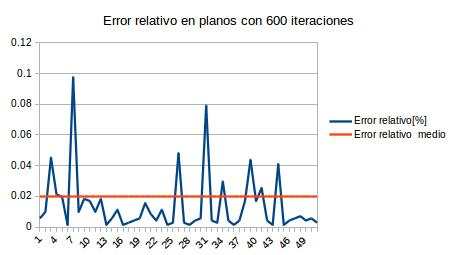
\includegraphics[width=10.5cm, height=3.4cm]{resultados/600_errRel.jpg}	
		\caption{Gráfica correspondiente al error relativo para el algoritmo RANSAC para detección de planos con 600 iteraciones.}

		\end{center}
	\end{figure}

	\begin{figure}[H]
		\begin{center}
		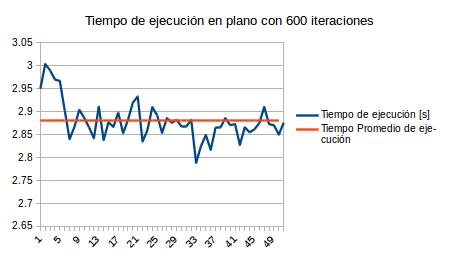
\includegraphics[width=12.5cm, height=6.0cm]{resultados/600_timeExec.jpg}
		\caption{Gráfica correspondiente al tiempo de ejecución para el algoritmo RANSAC para detección de planos con 600 iteraciones.}
		\end{center}
	\end{figure}

	Se tomaron 50 muestras para el algoritmo modificado con 200 iteraciones. los resultados se pueden observar en la siguiente gráfica.\\

	\begin{figure}[H]

		\begin{subfigure}[h]{.5\textwidth}
		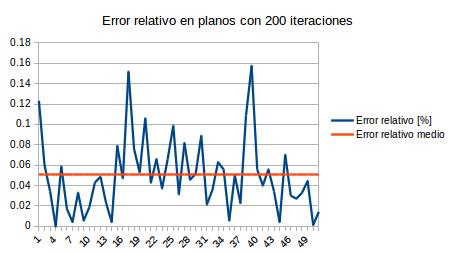
\includegraphics[width=8.5cm, height=5.0cm]{resultados/200_errRel.jpg}	
		\end{subfigure}%
		\begin{subfigure}[h]{.5\textwidth}
		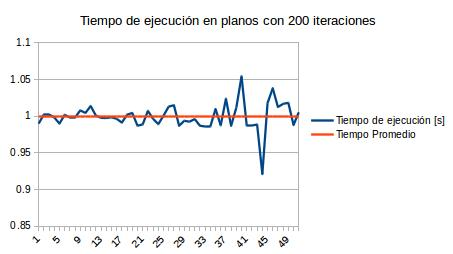
\includegraphics[width=8.5cm, height=5.0cm]{resultados/200_timeExec.jpg}
		\end{subfigure}
	
	\caption{Gráficas correspondientes al error relativo y tiempo de ejecución para el algoritmo RANSAC con 200 iteraciones.}

	\end{figure}

	Se continuó con el mismo principio para el algoritmo modificado con 100, 50, 30, 24 y 20 iteraciones respectivamente. Los resultados se pueden observar en las gráficas anexadas a continuación.\\


	\begin{figure}[H]

		\begin{subfigure}[h]{.5\textwidth}
		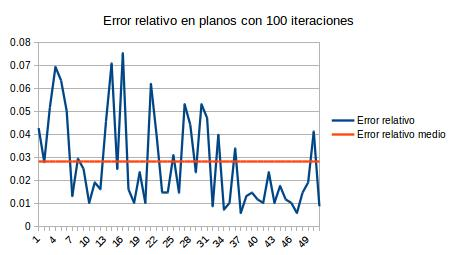
\includegraphics[width=8.5cm, height=5.0cm]{resultados/100_errRel.jpg}	
		\end{subfigure}%
		\begin{subfigure}[h]{.5\textwidth}
		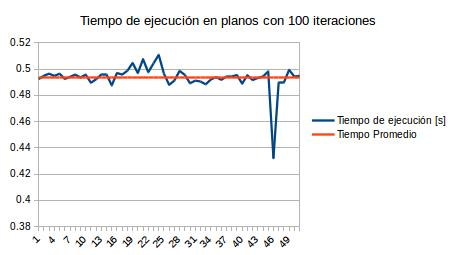
\includegraphics[width=8.5cm, height=5.0cm]{resultados/100_timeExec.jpg}
		\end{subfigure}
	
	\caption{Gráficas correspondientes al error relativo y tiempo de ejecución para el algoritmo RANSAC con 100 iteraciones.}

	\end{figure}

	\begin{figure}[H]

		\begin{subfigure}[h]{.5\textwidth}
		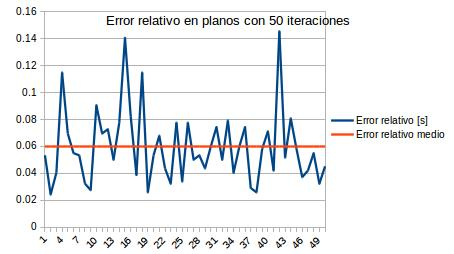
\includegraphics[width=8.5cm, height=5.0cm]{resultados/50_errRel.jpg}	
		\end{subfigure}%
		\begin{subfigure}[h]{.5\textwidth}
		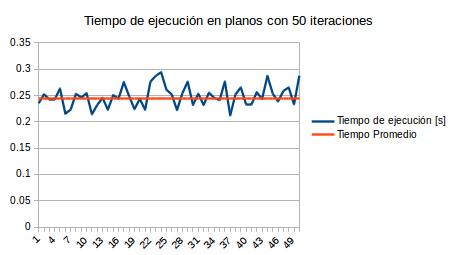
\includegraphics[width=8.5cm, height=5.0cm]{resultados/50_timeExec.jpg}
		\end{subfigure}
	
	\caption{Gráficas correspondientes al error relativo y tiempo de ejecución para el algoritmo RANSAC con 50 iteraciones.}

	\end{figure}

	\begin{figure}[H]

		\begin{subfigure}[h]{.5\textwidth}
		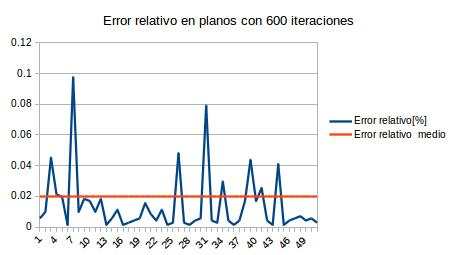
\includegraphics[width=8.5cm, height=5.0cm]{resultados/600_errRel.jpg}	
		\end{subfigure}%
		\begin{subfigure}[h]{.5\textwidth}
		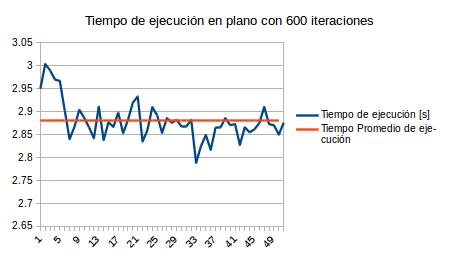
\includegraphics[width=8.5cm, height=5.0cm]{resultados/600_timeExec.jpg}
		\end{subfigure}
	
	\caption{Gráficas correspondientes al error relativo y tiempo de ejecución para el algoritmo RANSAC con 600 iteraciones.}

	\end{figure}

	\begin{figure}[ht!]

		\begin{subfigure}[h]{.5\textwidth}
		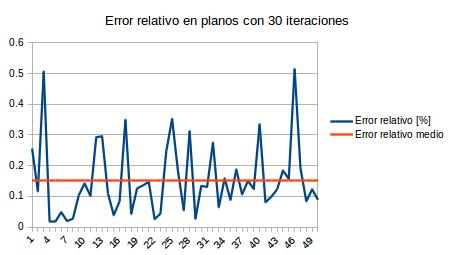
\includegraphics[width=8.5cm, height=5.0cm]{resultados/30_errRel.jpg}	
		\end{subfigure}%
		\begin{subfigure}[h]{.5\textwidth}
		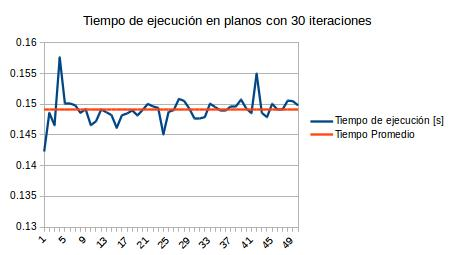
\includegraphics[width=8.5cm, height=5.0cm]{resultados/30_timeExec.jpg}
		\end{subfigure}
	
	\caption{Gráficas correspondientes al error relativo y tiempo de ejecución para el algoritmo RANSAC con 30 iteraciones.}

	\end{figure}

	\begin{figure}[H]

		\begin{subfigure}[h]{.5\textwidth}
		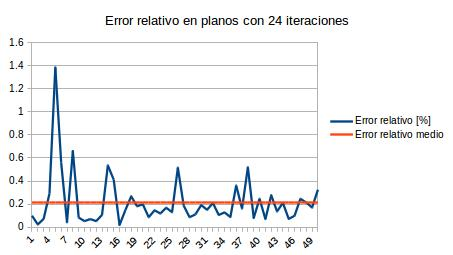
\includegraphics[width=8.5cm, height=5.0cm]{resultados/24_errRel.jpg}	
		\end{subfigure}%
		\begin{subfigure}[h]{.5\textwidth}
		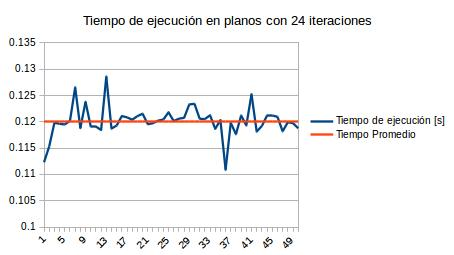
\includegraphics[width=8.5cm, height=5.0cm]{resultados/24_timeExec.jpg}
		\end{subfigure}
	
	\caption{Gráficas correspondientes al error relativo y tiempo de ejecución para el algoritmo RANSAC con 24 iteraciones.}

	\end{figure}

	\begin{figure}[H]
		\begin{subfigure}[h]{.5\textwidth}
		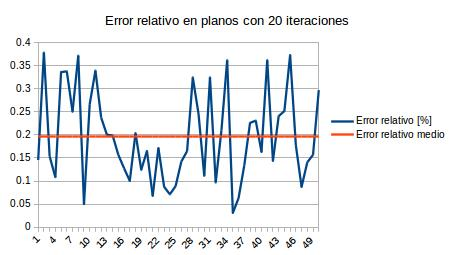
\includegraphics[width=8.5cm, height=5.0cm]{resultados/20_errRel.jpg}	
		\end{subfigure}%
		\begin{subfigure}[h]{.5\textwidth}
		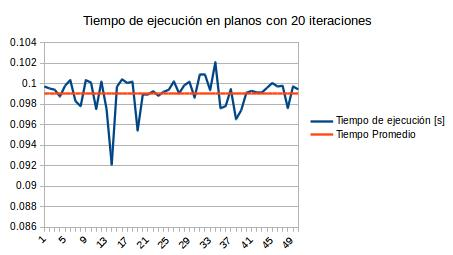
\includegraphics[width=8.5cm, height=5.0cm]{resultados/20_timeExec.jpg}
		\end{subfigure}
	\caption{Gráficas correspondientes al error relativo y tiempo de ejecución para el algoritmo RANSAC con 20 iteraciones.}
	\end{figure}

	Una vez que se obtuvo la información parcial de cada uno de estos eventos se realizó una tabla extra que agrupa la información del tiempo de ejecución promedio y el error relativo promedio contra el número de iteraciones del algoritmo. Se obtuvo la siguiente gráfica.\\

	\begin{figure}[H]
		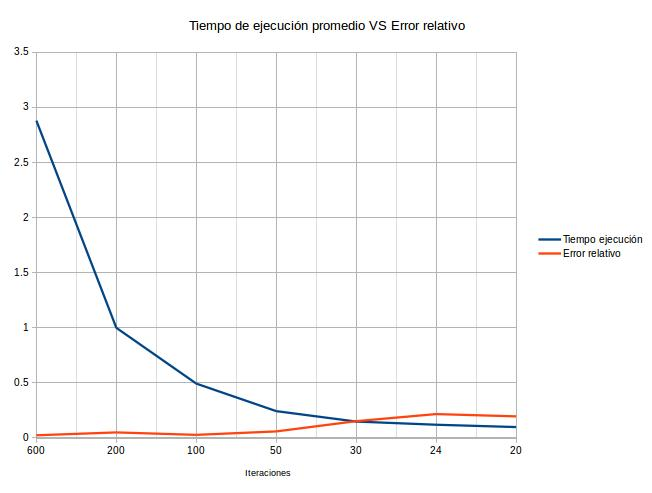
\includegraphics[width=14.5cm, height=8.0cm]{resultados/timeExec_errRel.jpg}
		\caption{Gráfica error relativo versus tiempo de ejecución para diferentes numeros de iteraciones.}
	\end{figure}


	Como podemos observar en la tabla 4.10 el error relativo presenta un incremento conforme se disminuye el número de iteraciones en el algoritmo. El tiempo de ejecución por su parte muestra un decremento conforme número de iteraciones disminuye. Dado este comportamiento de ambos parámetros resulta difícil encontrar un punto de equilibrio entre estas dos unidades de medición. Sin embargo observamos que tanto el error relativo como el tiempo de ejecución llegan a un valor estable, a partir del cual no aumentan o disminuyen significativamente. La gráfica 4.10 nos sugiere que este punto está en un número de iteraciones entre 30 y 24.\\ 



	\subsection{Comparación exactitud y rapidez}
	Para este conjunto de pruebas se comparó el algoritmo desarrollado en el presente trabajo contra el implementado acualmente en el robot de servicio Justina. Reportado en el trabajo de tesis Jesus Cruz Navarro. [**REFFF].\\

	Las pruebas se desarrollaron de la siguiente manera. Con la estructura de comunicación que permite ROS se implementaron dos servicios para encontrar planos: el desarrollado en este trabajo de tesis y el algortimo ya implementado. Se obtuvo la información de profundidad con el sensor RGB-D Kinect está infromación de compartió a traves de un tópico al cual ambos servicios se encontraban suscritos. De esta manera nos aseguramos de contar con la misma información en ambos algoritmos para poner a prueba la velocidad de ejecución y la precisión de algortimo.\\

	***Librería en C para medir obtener pulsos de reloj.\\


	En cuanto a la medidad de precisión del algoritmo continuamos suponiendo un plano horizontal del cual conocemos su altura; por tanto podemos conocer la ecuación del plano horizontal a esa altura. Probamos el algortimo para ese modelo y observamos la cantidad de puntos que entran en ese modelo, tomando este resultado como el ideal. Posteriormente se pusieron en funcionamiento ambos algoritmos midiendo la cantidad de puntos en los modelos obtenidos y comparadolos con el número de puntos ideal. Este evento se iteró una cantidad aproximada de 80 veces.\\


	Posteriormente calculamos el error relativo entre el modelo ideal y cada uno de los algoritmos. Como se muestran en la gráfica siguiente.\\


	La tabla \ref{t_result:1} resume los resultados obtenidos durante las pruebas.\\

	\begin{table}[h!]
	\centering 
	\begin{tabular}{ |p{6.5cm}||p{2.1cm}|p{2.1cm}|  }
	 \hline
	 \multicolumn{3}{|c|}{ Resultados algoritmo RANSAC } \\
	 \hline
	 \multicolumn{3}{|c|}{ Número de iteraciones: 1000}\\
	 \hline
	 \multicolumn{3}{|c|}{ Distancia miníma al modelo: 0.02[m]}\\
	 \hline
	                               &  Anterior     &	Actual \\
	 \hline
	 Tiempo promedio de ejecución  &  96.24[ms]    &   701.5[ms]\\
	 \hline
	 Error relativo promedio       &  39.95        &    8.78\\
	 \hline
	\end{tabular}
	\caption{Comparación de resultados de RANSAC para planos.}
	\label{t_result:1}
	\end{table}


	Con la información de que se ha reflejado en la tabla \ref{t_result:1} se puede deducir que la nueva implementación del algoritmo RANSAC con 1000 iteraciones y una distancia miníma al modelo de 0.02[m] es más lenta pero con menor error relativo. La diferencia de 605[ms] puede llegar a ser significativa si se requiere ejecutar el algoritmo iterativamente, sin embargo el común de las pruebas en ambientes del hogar no suelen requerir este tipo de acciones.\\  




%%%%%%%%%%%%%%%%%%%%%%%%%%%%%%%%%%%%%%%%%%%%%%%%%%%%%%%%%%%%%%%%%%%%
%%%%%%%%%     CARACTERISTICAS OBJETOS          %%%%%%%%%%%%%%%%%%%%%
	\section{Extracción de objetos y sus características}
	En lo que respecta a la extracción de objetos y sus características se procedió a realizar una caracterización de la misma. Para ello se realizaron un total de 100 eventos para cada uno de los 5 objetos diferentes: un control para videojuegos de forma irregular, una caja de cereal, un envase de jugo, un envase de bebida láctea y una barra de chocolate. Como información de interés se compararón las medidas de altura de los objetos. Puesto que el algoritmo previo tambien hacía una estímación de la altura de los objetos se compararon los resultados de ambos algoritmos. Como elementos de medida signiticativos se tomaron medida de tendencia central (valor esperado del dentroide) y como medida de dispersión se tomó la varianza. A continuación se presentan los resultados obtenidos de las mediciones realizadas.\\

	\begin{figure}[H]
		\centering
		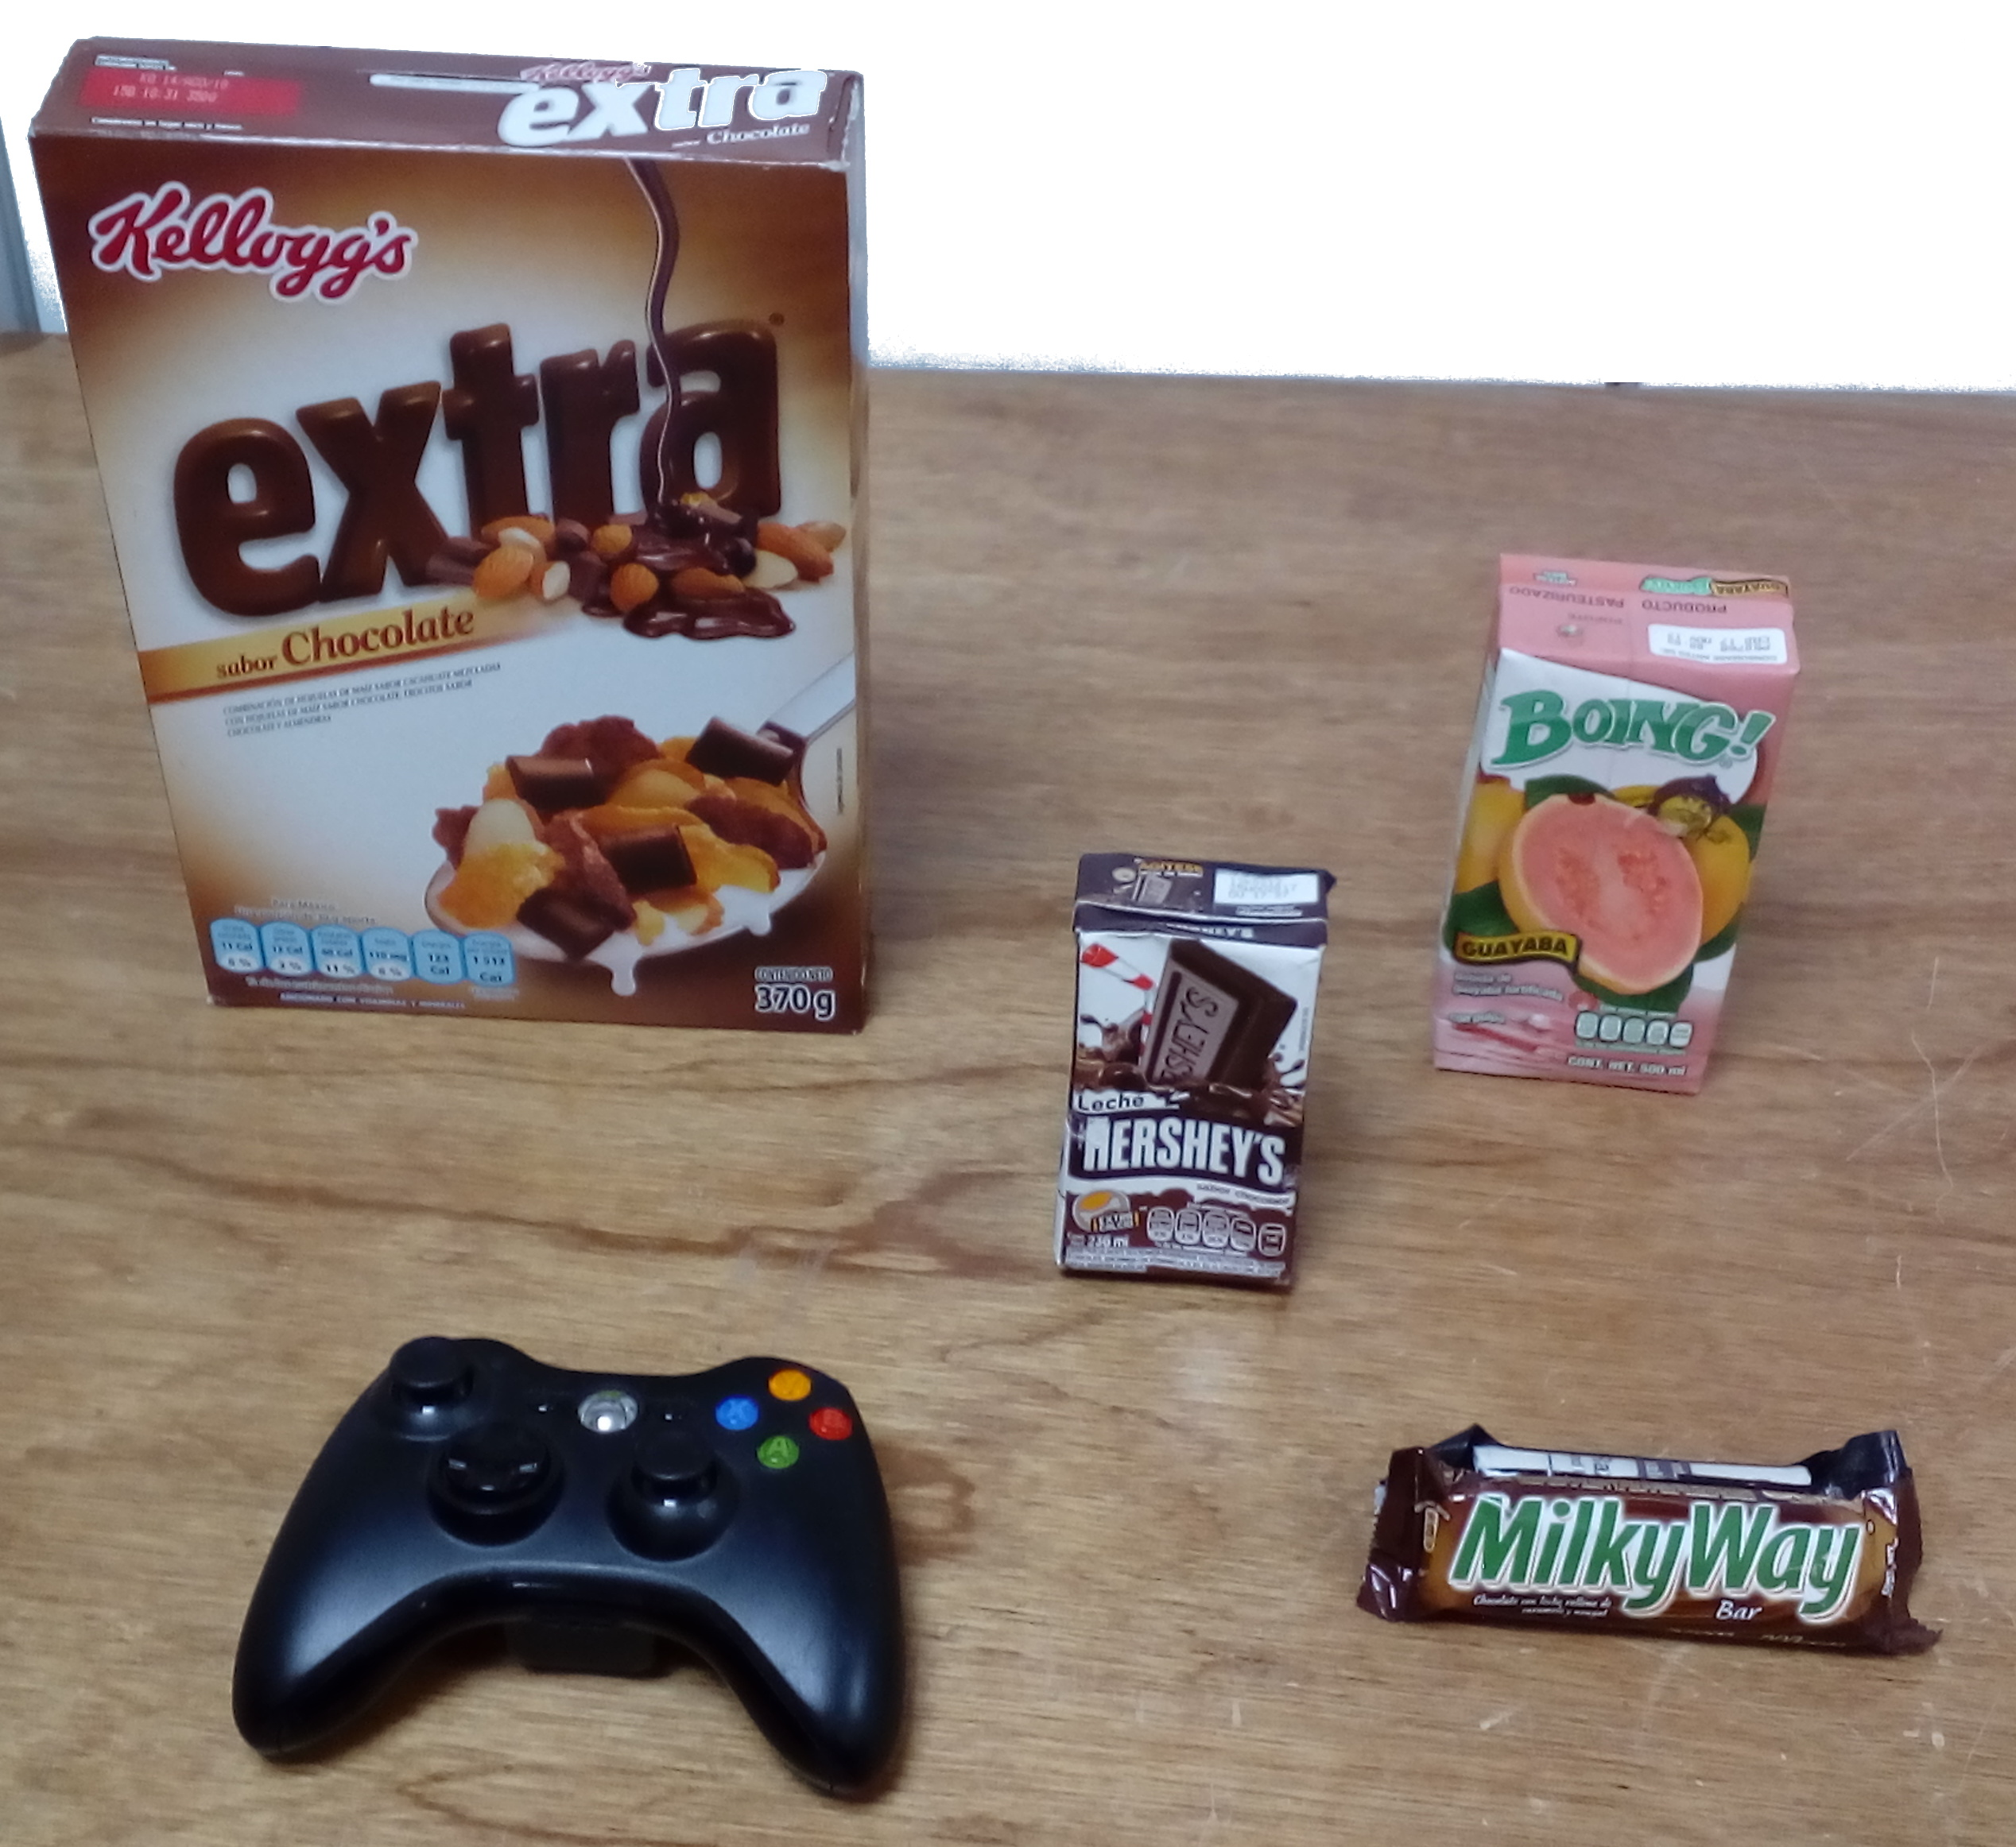
\includegraphics[scale=0.06]{objs_real/objects_2.jpg}	
		\caption{Fotografia de los objetos utilizados en las pruebas de cálculo de alturas y de manipulación de objetos.}
		\label{fig:objectsComplete}
	\end{figure}


	\subsection{Estímación de alturas}

	\begin{figure}[H]
		\begin{subfigure}[h]{.5\textwidth}
		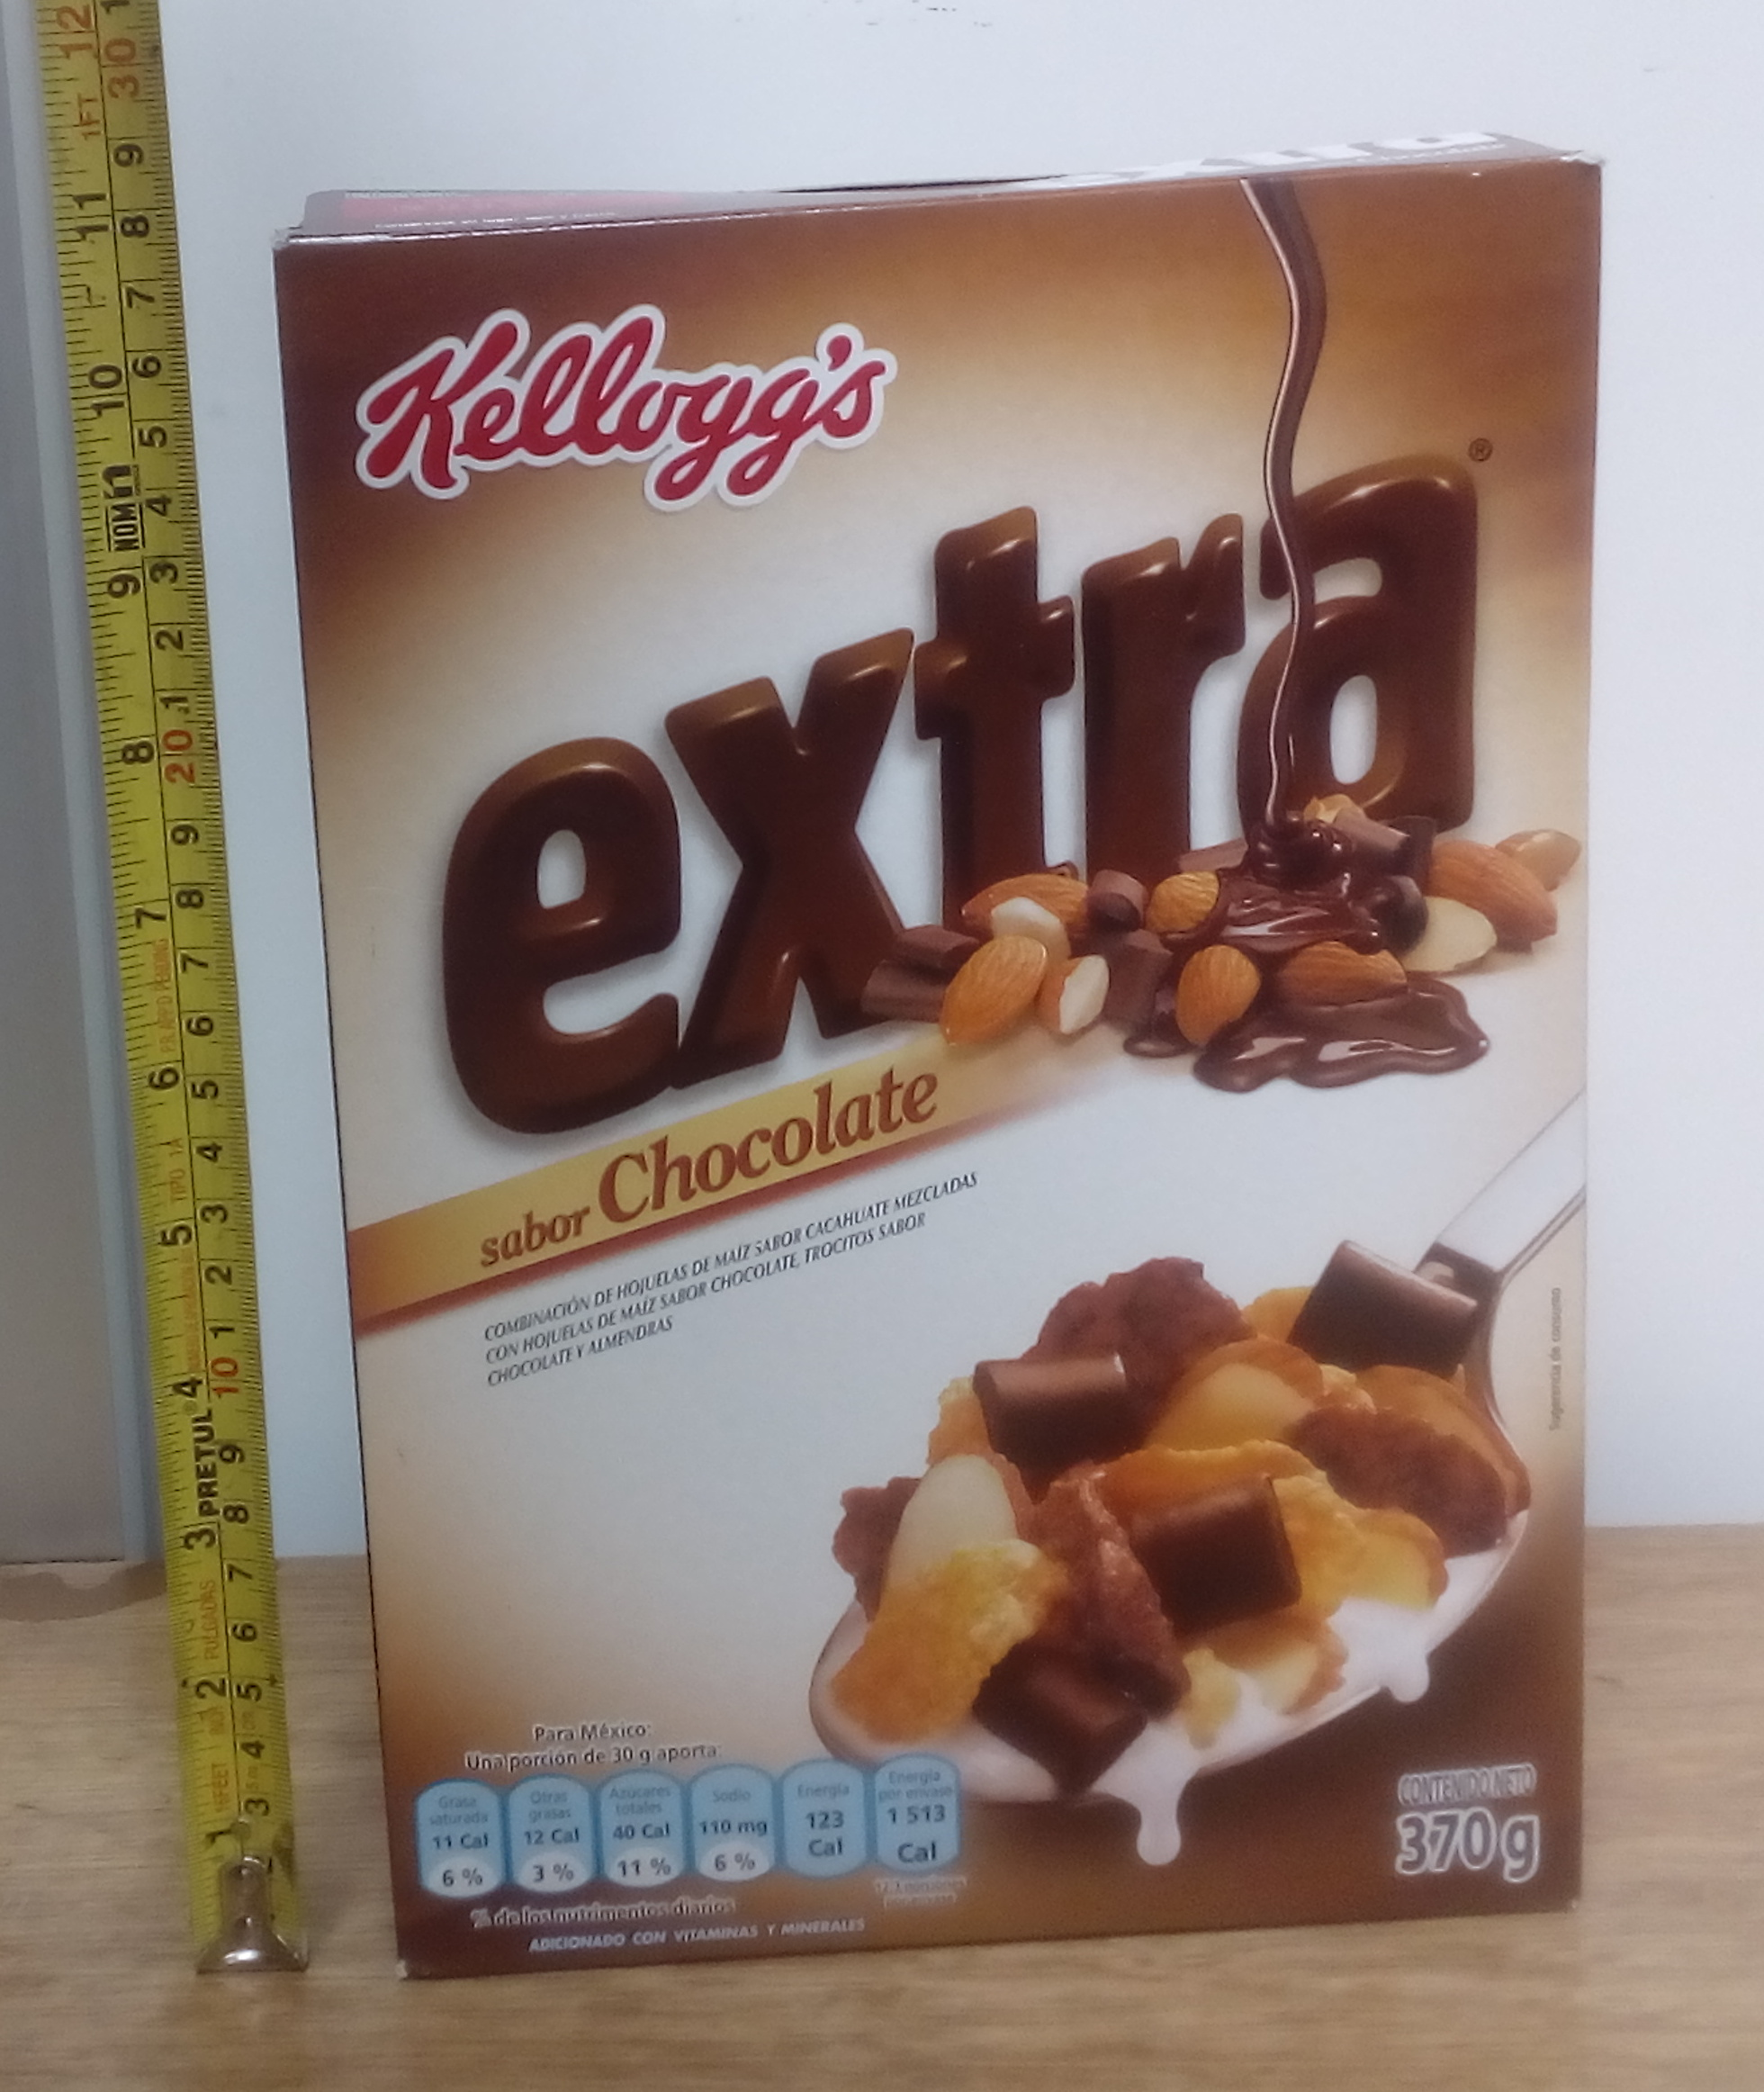
\includegraphics[scale=0.06]{objs_real/cerealBoxHeight.jpg}	
		\end{subfigure}%
		\begin{subfigure}[h]{.5\textwidth}
		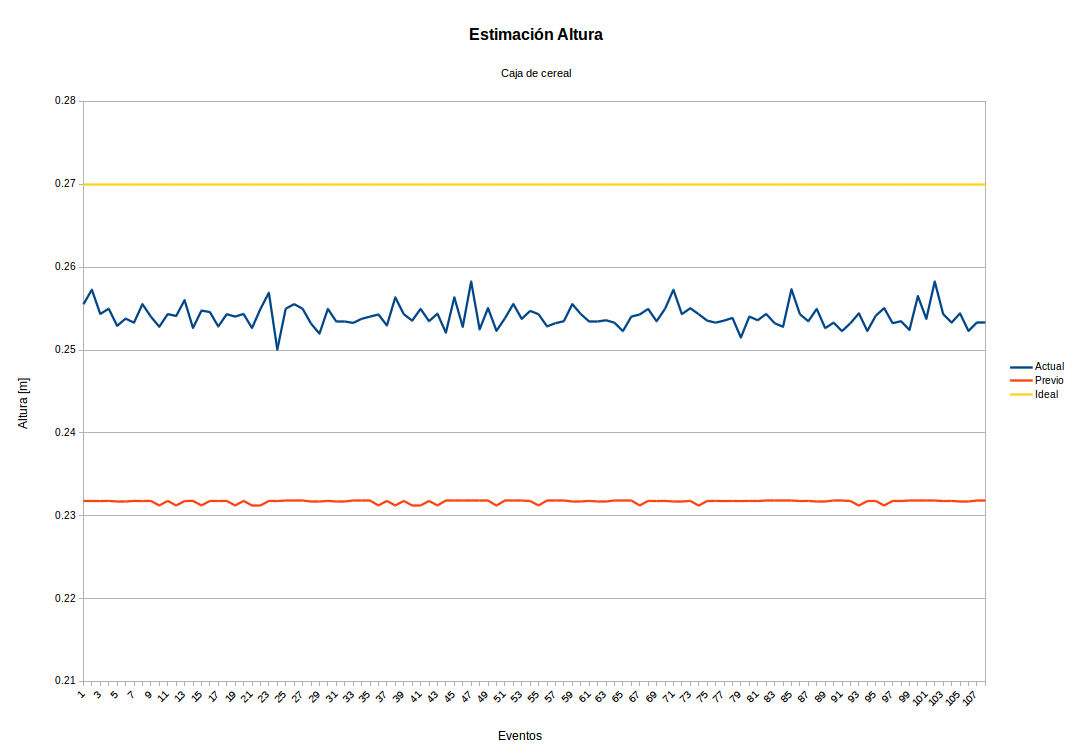
\includegraphics[scale=0.35]{resultados/cerealAltura.png}	
		\end{subfigure}
		\caption{Gráficas de estímaciones de alturas para una caja de cereal. La altura real del objeto (amarillo), la altura estímada con el algoritmo previo (rojo) y la estimación actual (azul).}
		\label{fig:mesh1}
	\end{figure}

	\begin{figure}[H]
		\begin{subfigure}[h]{.5\textwidth}
		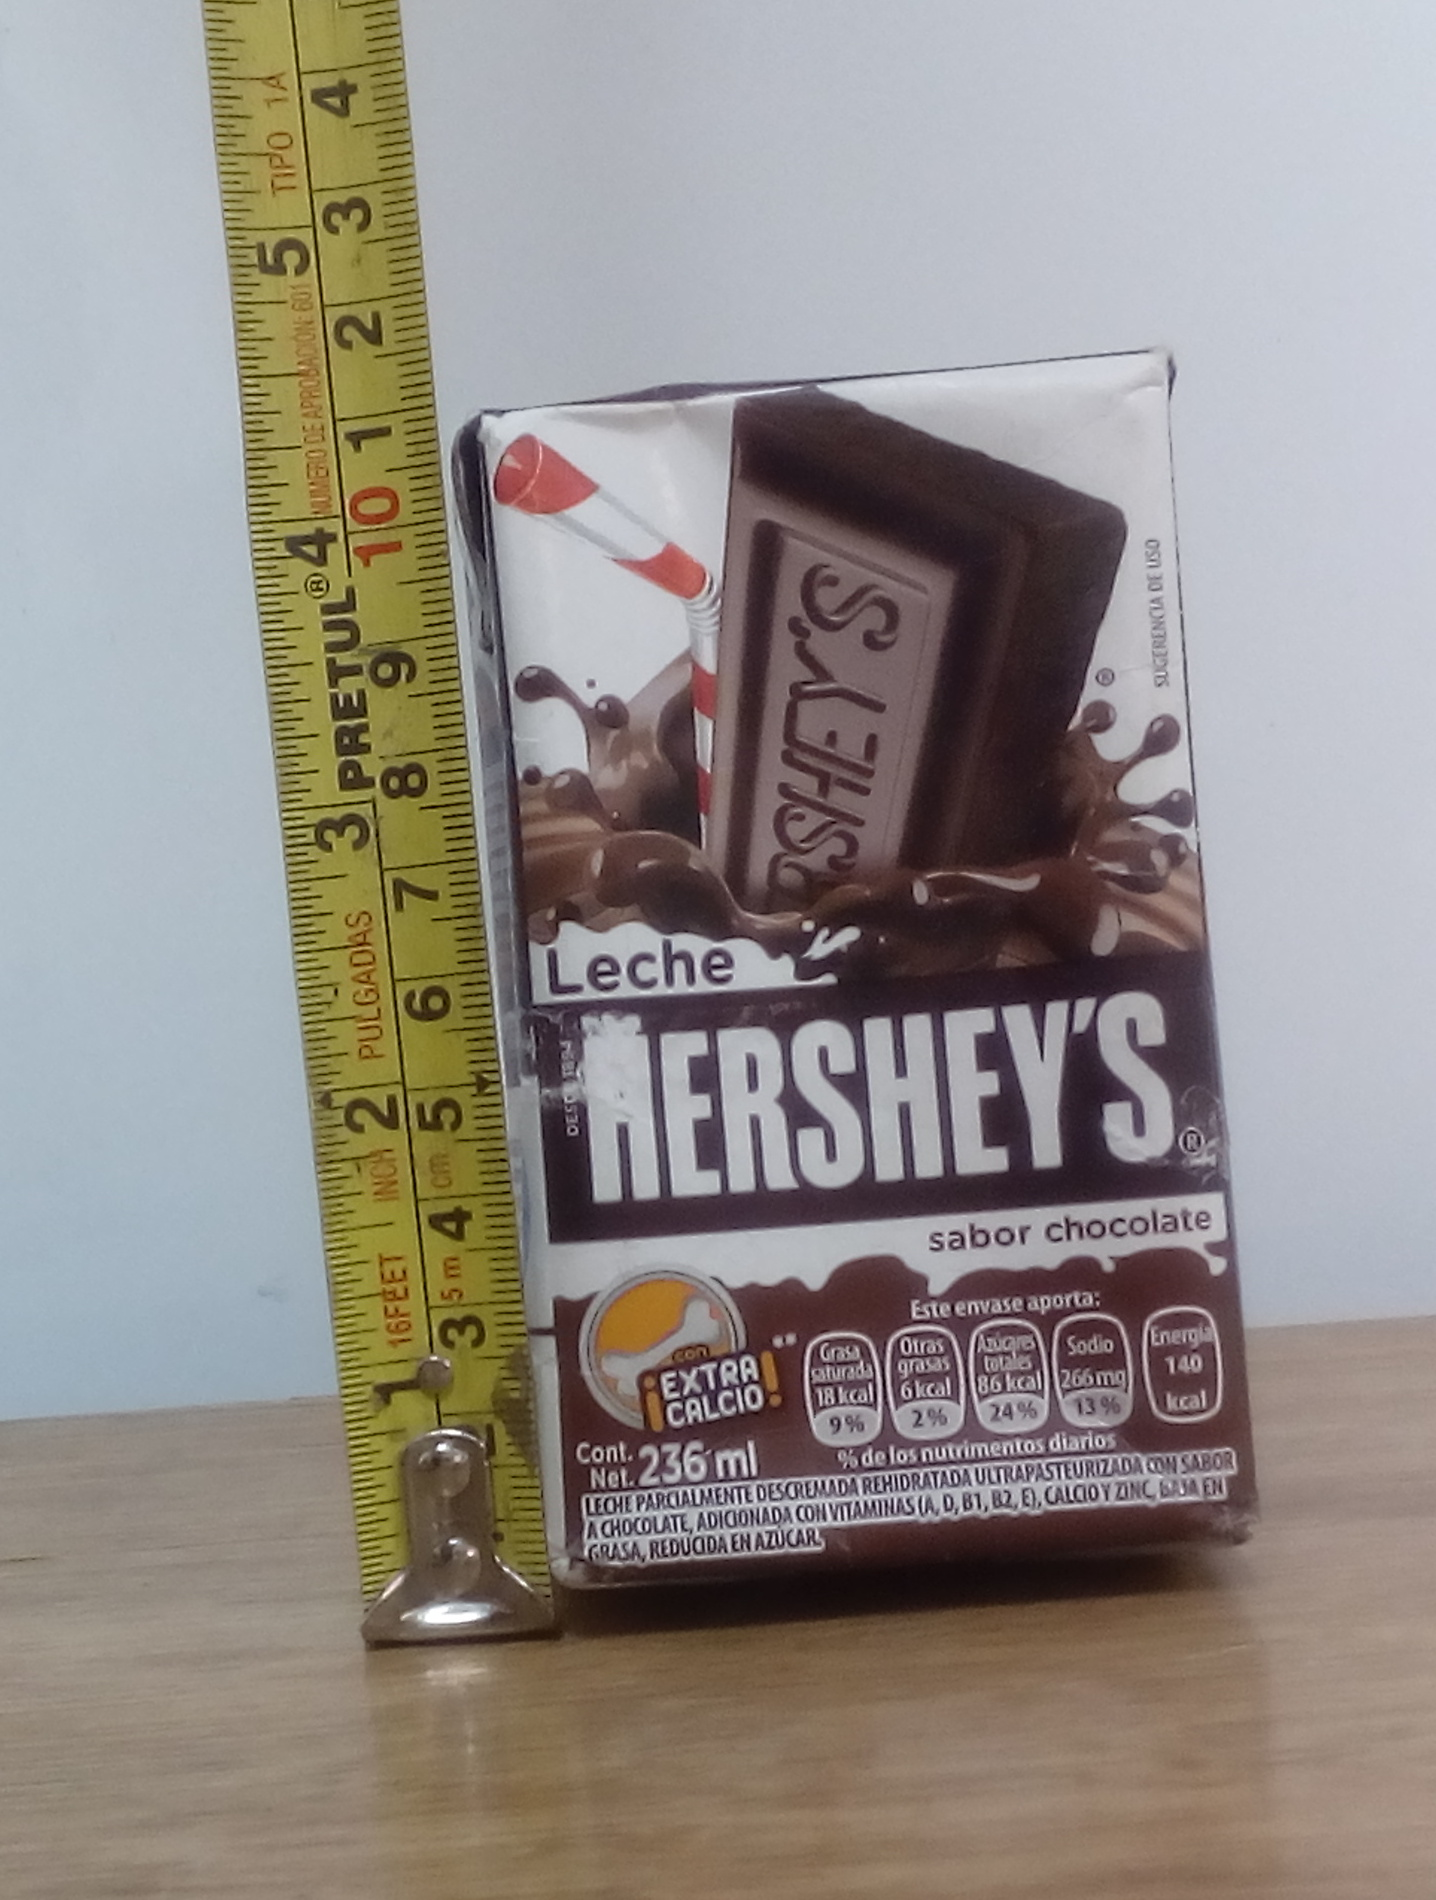
\includegraphics[scale=0.08]{objs_real/milkHeight.jpg}	
		\end{subfigure}%
		\begin{subfigure}[h]{.5\textwidth}
		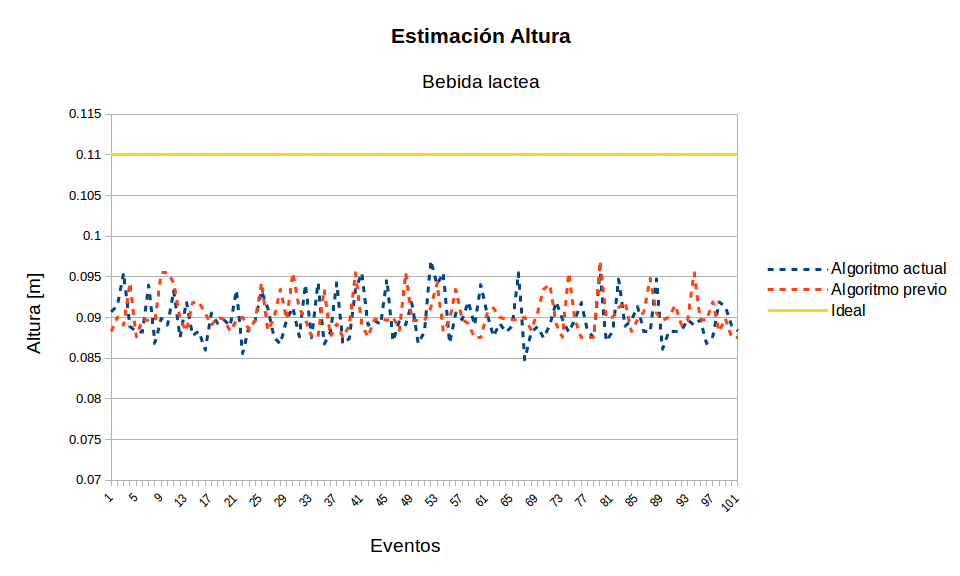
\includegraphics[scale=0.20]{resultados/lecheAltura.png}	
		\end{subfigure}
		\caption{Gráficas de estímaciones de alturas para un envase de leche. La altura real del objeto (amarillo), la altura estímada con el algoritmo previo (rojo) y la estimación actual (azul).}
		\label{fig:mesh1}
	\end{figure}

	\begin{figure}[H]
		\begin{subfigure}[h]{.5\textwidth}
		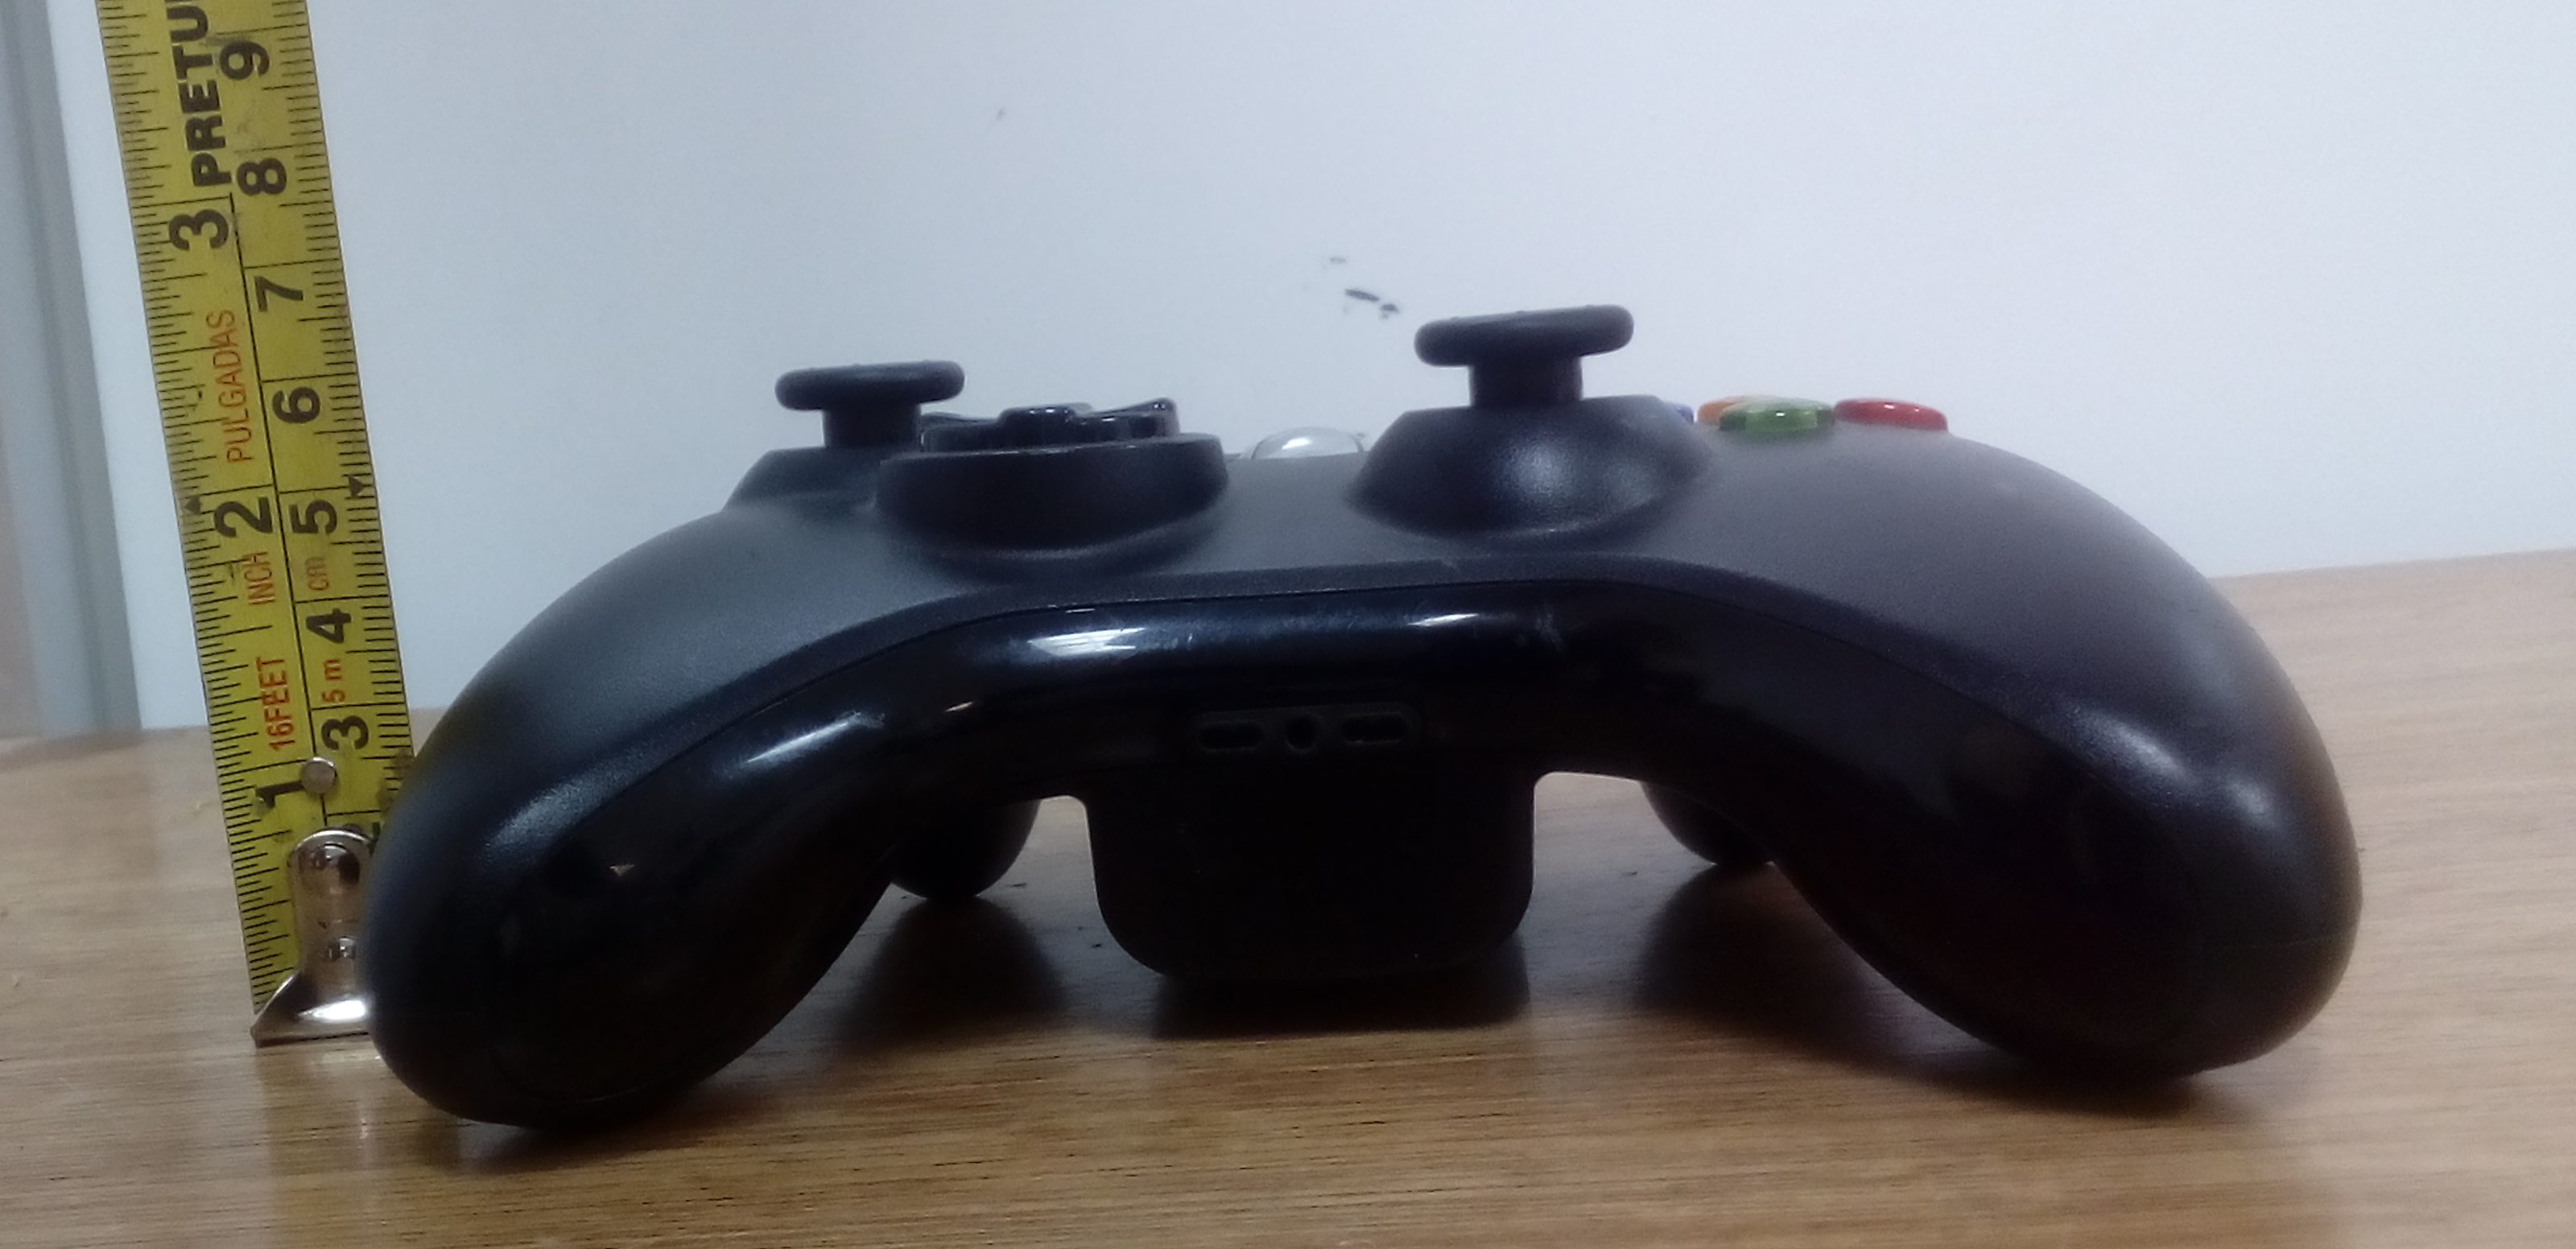
\includegraphics[scale=0.06]{objs_real/joystickHeight2.jpg}	
		\end{subfigure}%
		\begin{subfigure}[h]{.5\textwidth}
		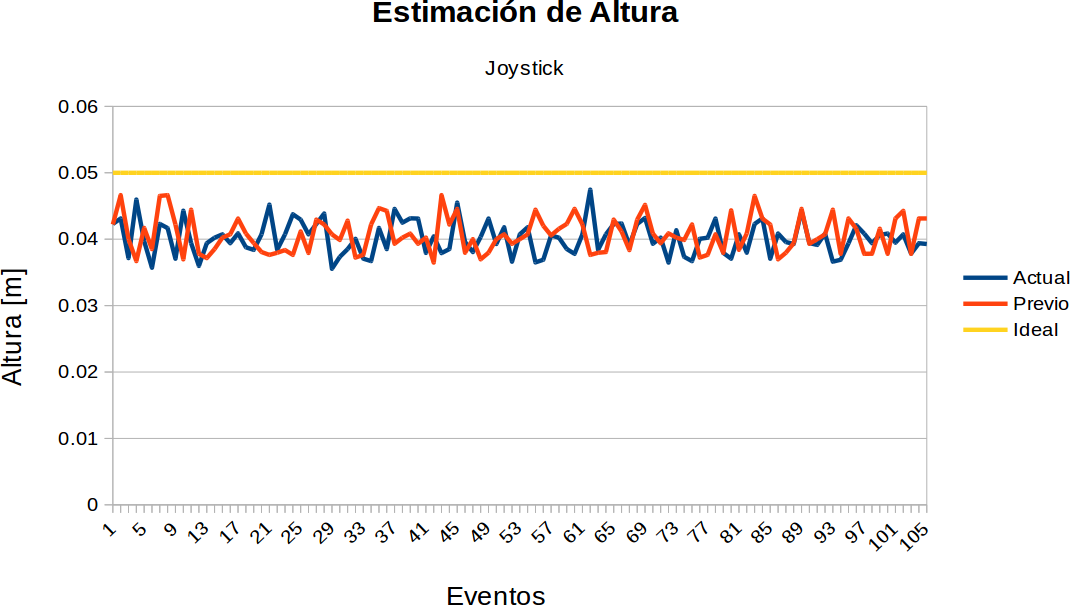
\includegraphics[scale=0.20]{resultados/joystickAltura.png}	
		\end{subfigure}
		\caption{Gráficas de estímaciones de alturas para un control de videojuegos. La altura real del objeto (amarillo), la altura estímada con el algoritmo previo (rojo) y la estimación actual (azul).}
		\label{fig:mesh1}
	\end{figure}

	\begin{figure}[H]
		\begin{subfigure}[h]{.5\textwidth}
		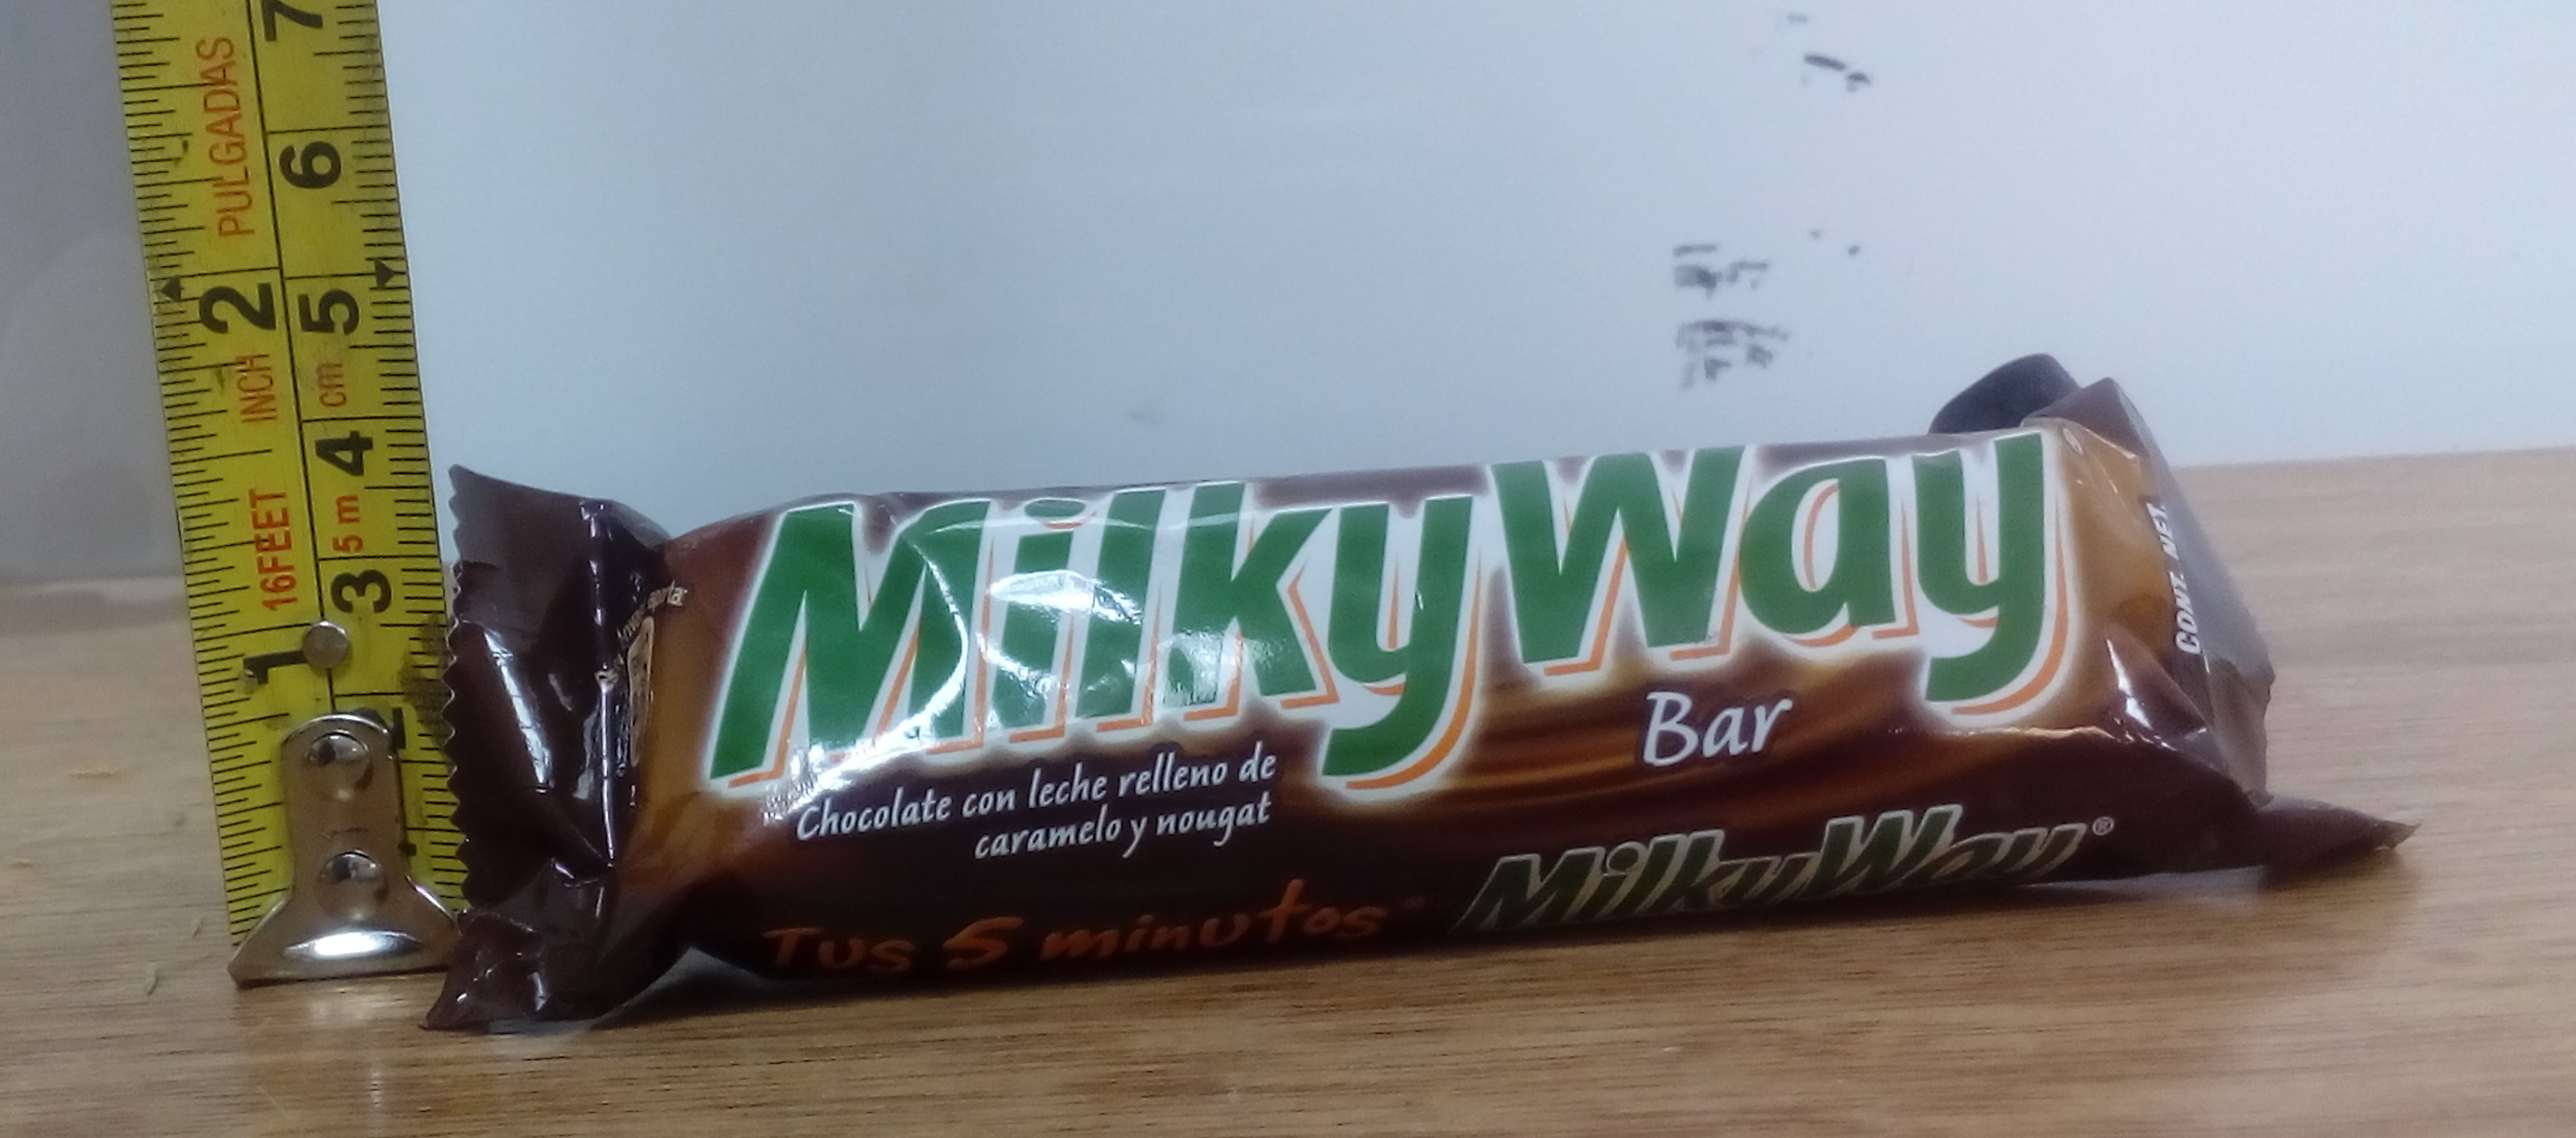
\includegraphics[scale=0.06]{objs_real/chocolateHeight2.jpg}	
		\end{subfigure}%
		\begin{subfigure}[h]{.5\textwidth}
		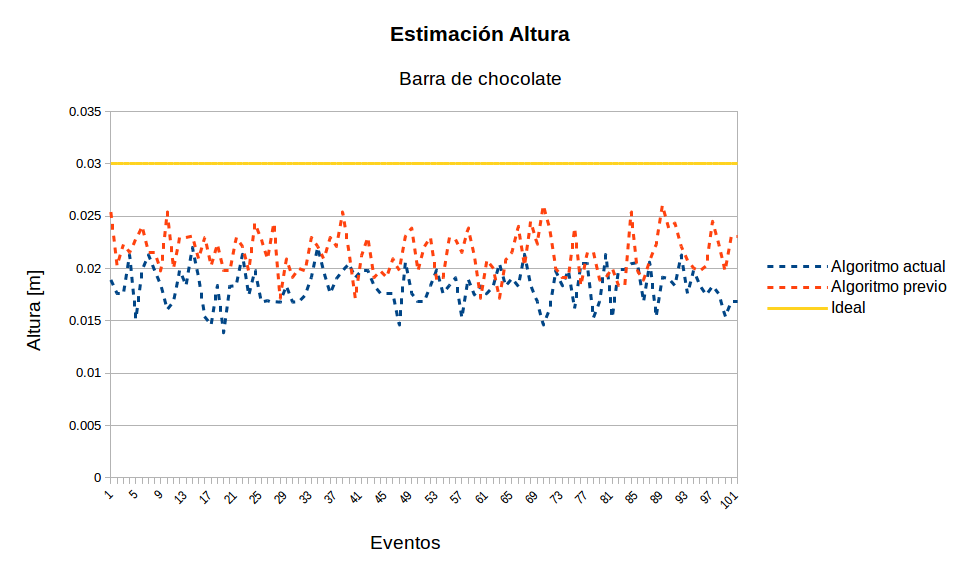
\includegraphics[scale=0.20]{resultados/chocolateAltura.png}	
		\end{subfigure}
		\caption{Gráficas de estímaciones de alturas para una barra de chocolate. La altura real del objeto (amarillo), la altura estímada con el algoritmo previo (rojo) y la estimación actual (azul).}
		\label{fig:mesh1}
	\end{figure}

	\begin{figure}[H]
		\begin{subfigure}[h]{.5\textwidth}
		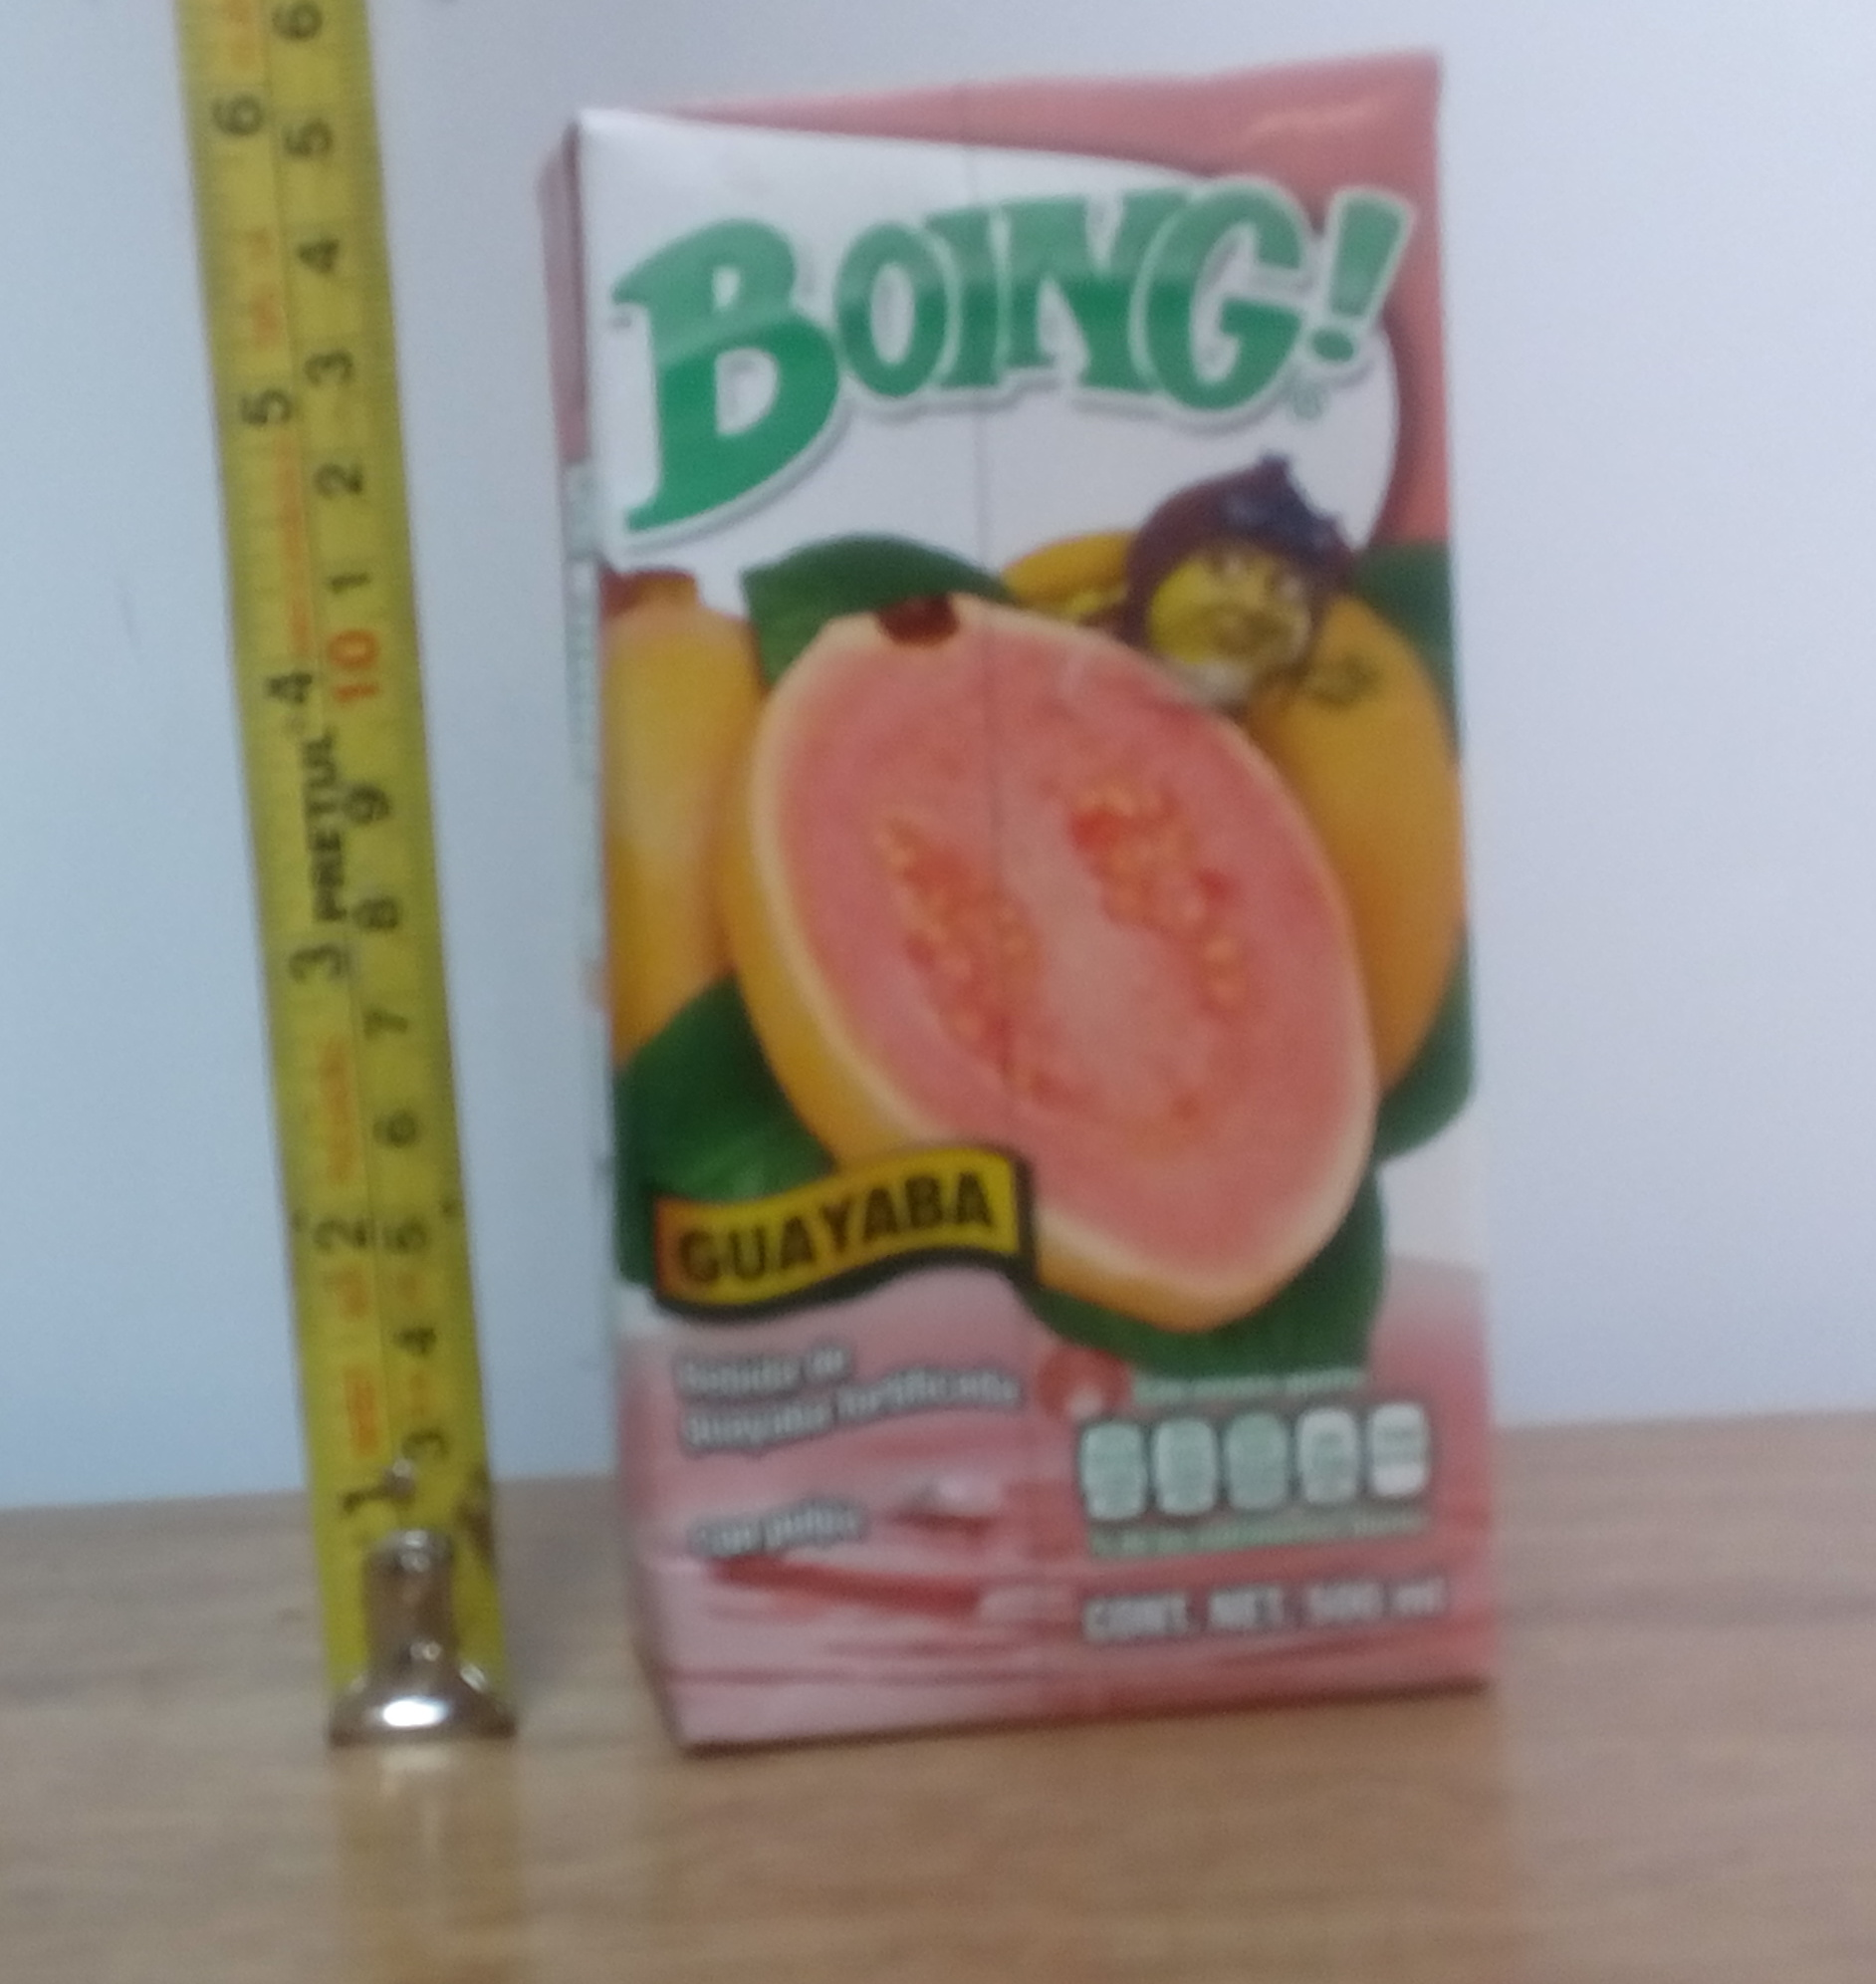
\includegraphics[scale=0.06]{objs_real/jugoHeight.jpg}	
		\end{subfigure}%
		\begin{subfigure}[h]{.5\textwidth}
		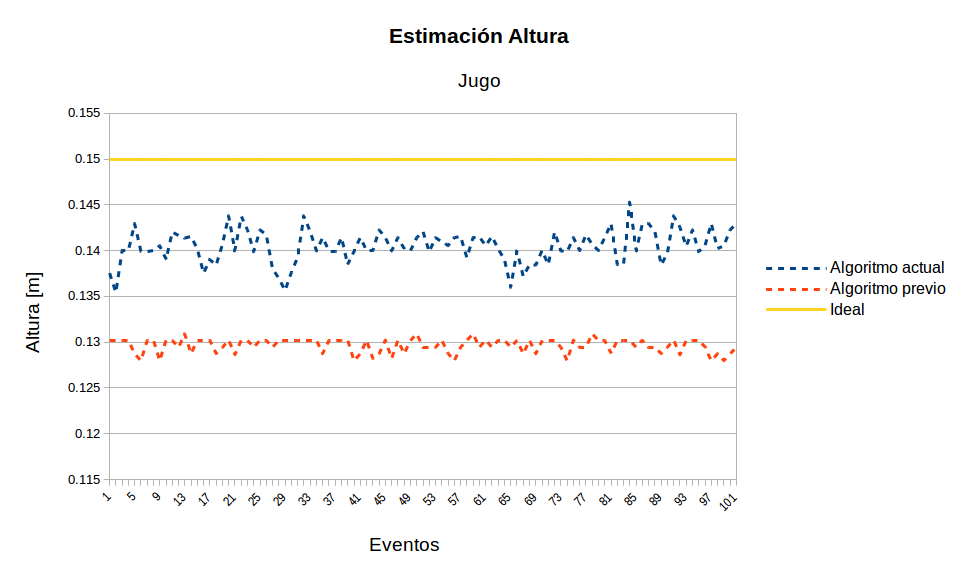
\includegraphics[scale=0.20]{resultados/jugoAltura.png}	
		\end{subfigure}
		\caption{Gráficas de estímaciones de alturas para un envase de jugo. La altura real del objeto (amarillo), la altura estímada con el algoritmo previo (rojo) y la estimación actual (azul).}
		\label{fig:mesh1}
	\end{figure}

	\subsection{Adicición de la información de dimensiones de los objetos}


%%%%%%%%%%%%%%%%%%%%%%%%%%%%%%%%%%%%%%%%%%%%%%%%%%%%%%%%%%%%
%%%%%%%%% Cálculo de las orientaciones  %%%%%%%%%%%%%%%%%%%%
	\section{Cálculo de la orientación del objeto.}
		\subsection{Prueba de exactitud}



%%%%%%%%%%%%%%%%%%%%%%%%%%%%%%%%%%%%%%%%%%%%%%%%%%%%%%%%%%%
%%%%%%%%%% PRUEBAS DE GRASPEO CON INFORMACIÖN DEL ÁREA DE TRABAJO  %%%%%%%%%%%%
	\section{Estimación de las dimensiones del área de trabajo.}
		\subsection{Comparación en tiempo de ejecución de la tarea de manipulación con información del área de trabajo.}



%%%%%%%%%%%%%%%%%%%%%%%%%%%%%%%%%%%%%%%%%%%%%%%%%%%%%%%%%%%%%%%%%%%%%%%%%%%%%%
%%%%%%%%%% PRUEBAS GRASPEO CON DIFERENTES INFORMACIONES %%%%%%%%%%%%
	\section{Pruebas de manipulación con el robot real}
		\subsection{Pruebas de manipulación actual.}

	Las pruebas se realizaron en 10 eventos para cada uno de los 5 diferentes objetos.\\
	4 de ellos se realizaron con el objeto a 0 grados respeco al eje y del robot.\\
	2 ocasiones el objeto se encontraba a 45$^{\circ}$ respecto al eje y del robot.\\
	2 ocasiones el objeto se encontraba a -45$^{\circ}$ respecto al eje y del robot.\\
	2 ocasiones el objeto se encontraba a 90$^{\circ}$ respecto al eje y del robot.\\

	Esto para cada uno de los algoritmos con los cuales se cuenta. 

	****Gráficas de eventos, reslatando exitos-fracacsos



		\subsection{Pruebas de manipulación con información de la orientación.}
	Las pruebas se realizaron en 10 eventos para cada uno de los 5 diferentes objetos.\\
	4 de ellos se realizaron con el objeto a 0 grados respeco al eje y del robot.\\
	2 ocasiones el objeto se encontraba a 45$^{\circ}$ respecto al eje y del robot.\\
	2 ocasiones el objeto se encontraba a -45$^{\circ}$ respecto al eje y del robot.\\
	2 ocasiones el objeto se encontraba a 90$^{\circ}$ respecto al eje y del robot.\\

	Esto para cada uno de los algoritmos con los cuales se cuenta. 

	****Gráficas de eventos, reslatando exitos-fracacsos



	\subsection{Pruebas de manipulación con información de la orientación e información de dimensiones..}
	Las pruebas se realizaron en 10 eventos para cada uno de los 5 diferentes objetos.\\
	4 de ellos se realizaron con el objeto a 0 grados respeco al eje y del robot.\\
	2 ocasiones el objeto se encontraba a 45$^{\circ}$ respecto al eje y del robot.\\
	2 ocasiones el objeto se encontraba a -45$^{\circ}$ respecto al eje y del robot.\\
	2 ocasiones el objeto se encontraba a 90$^{\circ}$ respecto al eje y del robot.\\

	Esto para cada uno de los algoritmos con los cuales se cuenta. 

	****Gráficas de eventos, reslatando exitos-fracacsos




%%%%%%%%%%%%%%%%%%%%%%%%%%%%%%%%%%%%%%%%%%%%%%%%%%%%%%%%%%%%
%%%%%%%%%		Conclusiones           %%%%%%%%%%%%%%%%%%%%%
\chapter{Conclusiones} 
	Partiendo de la información obtenida de los resultados podemos concluir que un algoritmo RANSAC con un umbral de 0.02 [m] y un número de 1000 iteraciones nos ayudará a encontrar la ecuación de un plano así como una lista de puntos pertenecientes al mismo. Esta impletenación tomará 8 veces más tiempo que la implementación actual pero reducirá el error relativo respecto al modelo real de un 39.9\% al 8.83\%.\\

